
\begin{frame}[t]{SNARC (1951)} 

A first neural net machine, \gls{snarc}, 
was built by \gls{Minsky} and \gls{Edmonds} in 1951.

\begin{columns}
    \begin{column}{0.45\textwidth}
      They design of \gls{snarc} drew inspiration from the work of 
      \gls{McCulloch} and \gls{Pitts} on
      artificial neurons.           
     \begin{center}
        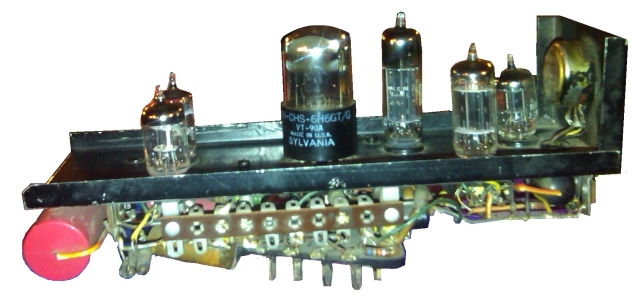
\includegraphics[width=0.99\textwidth]
        {./images/snarc/gregoryloan_snarc_hebbsynapse.png}\\
     {\scriptsize 
      A photograph by Gregory Loan of the only surviving \gls{snarc} neuron.\\
      \color{col:attribution} 
      Photo reproduced from \cite{CyberneticZoo:1951MazeSolver}}\\
     \end{center}
    \end{column}
    \begin{column}{0.55\textwidth}
       \begin{itemize} 
        \item
        \gls{snarc} was a randomly connected network 
        of about 40 neurons (Hebb synapses).
        \item
        Each neuron had a short-term memory and a long-term memory.
        \item
        The machine was trained by navigating a virtual maze 
        (i.e. \gls{snarc} was a "mechanical rat").
        \item
        Actions resulting to a positive reward (provided manually 
        by an operator), engaged a chain that turned a potentiometer 
        (whose setting was analogous to a weight in modern digital networks).
       \end{itemize}
    \end{column}
\end{columns}

\end{frame}